\section{Задание 4}

\begin{enumerate}
    \item Построить датчик распределения Коши. 
    \item На основе датчика распределения Коши с помощью метода фон Неймана построить датчик стандартного нормального распределения. При помощи функции normal probabitity plot убедиться в корректности построенного датчика и обосновать наблюдаемую линейную зависимость.
    \item Сравнить скорость моделирования стандартного нормального распределения в заданях 3 и 4.
\end{enumerate}

\subsection{Датчик распределения Коши}
    Распределение Коши~--- асбсолютно непрерывное распределение с функцией 
    распределения $F(x) = \frac{1}{2} + 
    \frac{1}{\pi}\arctg(\frac{x-x_0}{\gamma})$.

    Как и в пункте \ref{exp_section} воспользуемся методом 
    обратной функции:
    \begin{equation*}
        \xi \sim F^{-1}(\eta),
    \end{equation*}
    где $\eta \sim \mathrm{U}(0,1)$, 
    $F^{-1}(y)~=~x_0+\gamma\tg[\pi(x-\frac{1}{2})]$.

    Пример результата работы полученного датчика представлен на рис. 
    \ref{cauchy}.

    \begin{figure}[tbp]
        \centering
        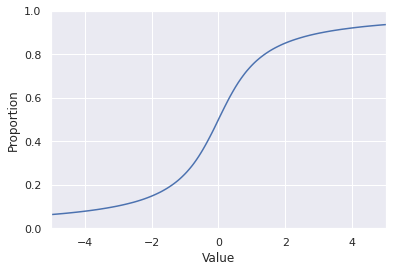
\includegraphics[width=0.5\textwidth]{resources/task4_cauchy.png}
        \caption{Э.ф.р. датчика Коши}
        \label{cauchy}
    \end{figure}

\subsection{Датчик стандартного нормального распределения 2} \label{4.2}
    Будем генерировать стандартную нормальную случайную величину методом 
    Фон-Неймана используя стандартное распределение Коши 
    ($\eta \sim \mathrm{Cauchy}(0,1)$) и распределение Бернулли.

    Требуемая выборка $\{X_i\}_{i=1}^n$ получается следующим образом. Для очередного $i$
    генерируется некоторое значение $x$ из закона $\eta \sim \mathrm{Cauchy}(0,1)$
    до тех пор, пока результат проведенного затем испытания Бернулли $\nu(x)$ с 
    вероятностью успеха $\frac{\sqrt{e}}{2} e^{-\frac{x^2}{2}} (x^2+1)$ не 
    будет положительным. Тогда значение элемента выборки $X_i$ принимается 
    равным $x$.

    Формула вероятности успеха в испытании Бернулли возникает как отношение
    "вероятностей попадания в точку $x$"$~$моделируемого распределения 
    (нормального) и распределения с помощью которого моделируют 
    (в нашем случае Коши), т.е. отношение плотностей 
    упомянутых распределений $\dfrac{p_1(x)}{p_2(x)}$. Здесь 
    $p_1(x) = \frac{1}{\sqrt{2\pi}}e^{-\frac{x^2}{2}}$, 
    $p_2(x) = \frac{1}{\pi}\frac{1}{x^2 + 1}$. Для ускорения работы 
    моделирующего алгоритма это отношение стараются приблизить к едиинце. 
    В данном случае это достигается домножением на коэффицинт $\dfrac{1}{k}$, 
    где $k = \sqrt{\dfrac{2\pi}{e}}$. В итоге получаем $p = 
    \dfrac{p_1(x)}{k p_2(x)} = \frac{\sqrt{e}}{2} e^{-\frac{x^2}{2}} (x^2+1)$.

    Для проверки корректности построенного датчика воспользуеся функцией 
    \texttt{scipy.stats.probplot}, которая строит теоретическую 
    (для стандартного нормального распределения) и эмпирическую 
    (для проверяемого распределения) функцию квантилей распределения. Поскольку 
    нормальное распредление для разных параметров линейно выражается через 
    стандратное, неудивительно что для разных $\mu$ и $\sigma$ график будет 
    меняться линейно. График для датчика стандартного нормального распределения 
    см. рис. \ref{normplot}.

    \begin{figure}[tbp]
        \centering
        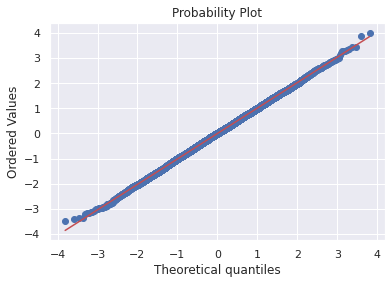
\includegraphics[width=0.5\textwidth]{resources/task4_normplot.png}
        \caption{}
        \label{normplot}
    \end{figure}

\subsection{Сравнение реализаций датчика стандартного нормального распределения}
    По результам 1000 запусков функций генерации выборки размера 1000 среднее
    время работы составляет
    \begin{itemize}
        \item $555\mu s \pm 28.6 \mu s$ для датчика из \ref{4.2}
        \item $83.6\mu s \pm 5.61 \mu s$ для датчика из \ref{3.4}
    \end{itemize}